% !TeX root = ../main.tex

\xchapter{智能光电系统实现与跟踪算法集成验证}{}
本章将详细介绍基于软硬件协同设计理念的智能光电系统整体实现方案,具体涵盖多光谱传感器采集、基于Nvidia Jetson和RK3588边缘计算平台的算法部署与优化,以及采用模块化设计的端侧全功能软件框架。为了确保系统中各模块间高效、可靠的数据交换与控制,本章专门设计了配套的轻量级通信协议,定义了传感器、计算单元与上位机之间的标准化数据接口。同时,开发了功能完善的上位机软件,集成了实时状态监控、算法参数调整、结果可视化以及视频与日志记录功能,为系统调试、性能评估和人机交互提供了直观友好的操作界面。其次,针对动态复杂环境中目标易丢失的难题,本章提出了面向边缘计算设备的融合重识别机制与自适应模板更新的抗遮挡长时目标跟踪算法,并将其集成到智能光电系统中,通过实际场景测试验证了其鲁棒性。本章工作不仅验证了算法的工程可行性,也为构建自主智能光电系统提供了从底层硬件、核心算法到交互软件的完整原型参考与实践依据。

\xsection{引言}{Introduction}
随着低空经济的蓬勃发展和无人机任务复杂度的不断提升,机载光电系统正经历着从“被动观测”到“主动感知”、从“功能单一”到“多任务智能”的全面角色转变。在信息化、网络化、智能化融合发展的背景下,现实环境呈现出高度动态、高度复杂、信息饱和的特征,对环境感知的实时性、准确性、自主性提出了更严格的要求。这一系列需求驱动机载光电系统向智能化方向发展。智能化是指系统具备从原始数据中自主提取信息、在复杂不确定环境下进行稳定推理、并依据任务目标做出及时响应或决策的闭环能力,最终目标是使光电系统成为具备一定“认知”能力的空中智能体,能够在最小化人工干预的情况下,独立完成从搜索、发现、识别、跟踪到评估的完整环节。然而,现有系统距离实现上述理想的、完整的“智能化”,仍存在显著的差距,主要体现在硬件与软件两个层面。

在硬件层面,机载平台,尤其是中小型无人机,对载荷有着严格的尺寸、重量、功耗和成本限制,这导致机载信息处理单元算力与内存带宽有限,与云服务器或大型地面站相比,存在数量级差距。这种有限的计算资源与当前先进的视觉算法对算力的庞大需求构成了直接矛盾,尤其对于参数量庞大、计算密集的Transformer模型。许多在实验室标准数据集上表现优异的算法,因其复杂的计算度和巨大的延迟,难以直接部署到机载平台进行实时推理。因此,现有的“智能”往往是一种被严重约束的智能,需要在算法性能与实时性之间做出艰难平衡,导致许多先进的感知能力在端侧无法充分发挥。另外,更深层次的制约源于机载环境严苛的功耗与热管理约束。即便在机载平台中采用了具有高算力的边缘计算模块,其性能也往往受到物理规律的严峻挑战。机载平台的电能供给极为有限。无人机续航直接依赖于机载电池,为所有载荷(包括飞控、传感器、通信与计算单元)分配固定的功率预算。一个在实验室中峰值功耗可达数十瓦的高性能计算模块,在机载环境下可能因超出功率预算而无法被允许持续运行在峰值状态。设计者通常被迫在其峰值性能和平均功耗之间做出权衡,通过软件或硬件手段设置功耗墙,这意味着硬件在其工作的大部分时间里都无法以其最大标称频率运行。其次,与功耗紧密相关的热管理问题在机载环境中尤为突出。计算芯片在高负载下产生的热量必须被有效散出,以防止芯片结温超过安全阈值导致降频、重启甚至永久损坏。然而,无人机紧凑的机体内通常缺乏空间部署大型主动散热系统(如风扇阵列或液冷回路),主要依赖有限表面积下的被动散热或风冷。在低空低速或悬停状态下,对流散热效率降低,极易导致热量积聚。因此,即使硬件模块在理论上具备高算力,在实际飞行中,其持续运算往往会迅速触发温度保护机制,迫使系统动态降频以控制温度,使得实际可持续的运算性能远低于标称峰值。这种由功耗与热约束导致的性能降级对于实际工程应用具有重大影响。许多在实验室标准数据集上、有充足散热保障的硬件平台上表现优异的复杂算法,一旦置于真实的机载环境,便会因计算单元的瞬时算力下降和频繁降频,而遭遇难以预测的性能波动和延迟激增。算法原本稳定的处理流水线被破坏,实时性指标急剧恶化。因此,现有的机载“智能”往往是一种被双重约束的智能:一是底层硬件资源的绝对不足,二是即使存在的硬件资源也因物理限制而无法全力输出。系统设计必须在算法理论性能、实时性要求、功耗上限与散热能力之间进行多维度的、艰难的平衡,这导致许多先进的感知模型在端侧无法充分发挥其潜力,甚至不得不为保障最基本的运行可靠性而牺牲精度与功能。

在软件与算法层面,现有系统更多地解决了“有无”问题,但与“智能”的本质要求尚有巨大差距。现有功能大多围绕单一、特定的任务(如“对指定类别的目标进行检测或跟踪”)进行优化。其算法流程往往是链式或并行的,检测、跟踪等模块相对独立,信息流动单向。算法模型通常在离线状态下用固定数据集训练完成,一旦部署,其参数和结构就已经固化。面对训练数据未充分涵盖的新环境、新目标类型或新型干扰,系统性能会急剧下降。
在特定数据集上取得高精度的算法,在实际复杂的使用环境中,其性能边界往往模糊不清。对于采用深度神经网络的算法,当其在边缘设备部署时,必须借助边缘芯片厂商提供的专用工具链(如NVIDIA的TensorRT、华为的CANN、瑞芯微RKNN等)对模型进行量化、编译与优化,以使其能在特定的异构计算硬件上高效执行。然而,这个过程,往往以牺牲一定的算法精度为代价,导致在标准数据集上评测出的高精度无法无损地转化到实际应用中。从FP32到FP16或INT8的量化,使可表示的数值分辨率急剧下降。对于特征图中表征微弱信号或精细结构的小数值,量化后可能归零或产生较大相对误差,直接影响对小目标、低对比度目标或目标边缘的感知精度。这些工具链为了极致性能,会将多个基础算子(如卷积、批归一化、激活)融合为一个复合算子,并进行内存访问优化。然而,这种融合有时会改变运算的微小数值顺序或精度,可能与原始训练时定义的数学行为存在细微偏差,在网络中被逐层放大,最终导致误检、漏检或跟踪漂移。因此,一个神经网络经过量化部署到机载边缘平台后,其实际性能存在不可避免的损失,这种损失使得算法在实际复杂环境下的性能边界更加模糊和脆弱。

本章的核心将从纯算法研究与理论分析,转向以实际部署与应用验证为导向的系统工程实践。具体而言,我们首先构建一套完整的软硬件协同设计架构,涵盖从多光谱传感器数据采集、到基于边缘计算设备的算法深度优化部署、再到模块化软件框架实现的全链路集成方案。进而,针对复杂动态场景中最具挑战性的目标持续跟踪问题,本章将提出并集成一种创新的抗遮挡长时跟踪算法,并通过实际场景测试,验证评估其在接近真实条件中的鲁棒性与实用性。最终,本章旨在打通从先进算法到可靠系统产品的关键路径,为智能光电系统的工程化与实战化提供一套经过验证的方法论与实例。



\xsection{智能光电系统整体架构与工作原理}{Overall Implementation Scheme of Intelligent Electro-Optical System}

% \xsubsection{系统组成及工作原理}{}
机载光电系统主要由红外分系统、可见光分系统、激光分系统、稳定跟踪分系统、系统控制分系统、图像处理分系统、和结构分系统等组成,其工作原理如图\ref{sys-arch}所示。从系统运行角度来说,各分系统是一个有机的整体,通过各分系统之间的协调工作实现相应的功能性能。从物理结构角度上说,光电系统有的分系统与其他分系统综合为一体,如红外分系统、可见光分系统等光机部件交织在一起,有的分系统是模块化。

\begin{figure}[H]
\centering
\includegraphics[width=\textwidth]{sys-arch.png}
\caption{机载光电系统组成框图}
\label{sys-arch}
\end{figure}

\xsubsection{红外分系统}{}
红外分系统是机载光电系统实现全天时全天候环境感知能力的主要传感器,由于它利用的是物体(目标/背景)自身发射的红外谱段的光线,可以完全不依赖周边环境的光源,是短波、微光以及激光等不可替代的光学探测通道,通常是光电系统的必备传感器。红外分系统主要由红外光学镜头、支撑光学镜组的精密光机结构、红外探测器、信息处理部件、视场切换机构、变焦机构等部件组成,如图\ref{ircam-sys}所示。红外分系统主要功能是对地面景物热辐射信息进行光电转换,输出视频信号给信息处理单元用于后续检测跟踪任务,同时为了适应不同环境下得到便于处理分析的图像,红外分系统具有电子变焦、黑白热切换、图像冻结、增益控制、偏置控制等功能。一般情况下,红外分系统在光电系统中是一个独立的组件,能够方便地进行更换,称为红外热像仪。有时红外光学光机部分与可见光光学、激光光学融合在一起形成一个十分复杂的光机构型,如共光路构型,瞄准吊舱多采用此种构型。

\begin{figure}[H]
\centering
\includegraphics[width=\textwidth]{ircam-sys.png}
\caption{红外分系统组成}
\label{ircam-sys}
\end{figure}

红外分系统在设计过程中主要考虑以下几个方面。
% \paragraph{波段选择}
红外系统的波长范围确定非常重要,同时工作波长也是系统总体指标之一。在红外分系统设计中,根据大气窗口可以选择中波(3-5μm)和长波(8-12μm)两个波段,具体波段的选择主要与目标和背景的辐射特性、大气传输特性和系统性能有关。设目标的辐射系数为$\varepsilon(\lambda,T)$,目标的积分辐射出射度为:
\begin{equation}
    M\left(\lambda_1-\lambda_2\right)=\int_{\lambda_1}^{\lambda_2} \varepsilon(\lambda, T) M_{\mathrm{eo}}(\lambda, T) \mathrm{d} \lambda
\end{equation}

根据维恩位移定律
\begin{equation}
    \lambda_mT=2897.8μm\cdot K
\end{equation}

由于目标辐射峰值波长与温度成反比,从辐射特性的角度分析,对于目标特征为高温物体的红外系统选用中波波段,对于目标特征为常温物体的红外系统选用长波波段。但红外系统波段的选择还要考虑使用环境,由于空气湿度对长波影响较对中波影响严重,对于海上高温高湿的环境一般选用中波红外系统。从实际应用角度,由于近几年中波红外制冷型探测器灵敏度得到了很大程度的提高,工艺稳定,同时制冷型长波红外探测器较中波红外探测器存在成本高、稳定性较差等问题,因此目前国外研制的光电跟瞄系统采用中波红外的比例很高,在具体设计中红外分系统的波段选择要根据实际系统的使用情况综合考虑。

\paragraph{光学设计}
红外光学镜头是保证系统光学性能的关键部件,在很大程度上影响着红外分系统的性能。在红外探测器确定后,系统总体设计中关于红外发现和识别距离的指标主要依靠光学设计保证。光学设计需要综合考虑视场大小、视场数量、焦距和传递函数等指标的要求,同时也要满足尺寸空间、重量、温度振动等环境条件的约束。

\paragraph{视场变换}
红外分系统一般设计两个以上光学视场,宽视场用于广域搜索潜在目标,窄视场用于分辨识别目标的轮廓细节。视场切换的实现一般采用两种光学构型,第一种采用轴向移动透镜实现视场切换,第二种采用切入/切出变倍镜组实现视场切换。

\paragraph{图像增强}
由于红外图像动态范围较大,在将其转换为适合人眼观察的模拟图像过程中,容易造成图像细节的缺失,影响人眼的观察效果。红外探测器输出的原始数据一般为16位,而显示器显示的图像数据一般为8位。现代红外相机通常在内部集成了一系列基础的图像增强与校正功能,优化输出图像的视觉质量,其中以非均匀性校正和坏点补偿为基础,消除由探测器像元响应差异引起的固定模式噪声,确保图像均匀性,同时,对传感器缺陷造成的图像中的亮点或暗点进行检测和补偿,随后,通过基于查找表的动态范围压缩与对比度增强算法,将宽广的原始灰度范围进行智能映射,有选择地拉伸感兴趣温区的对比度以凸显细节,抑制非关键区域的灰度变化。同时,为优化主观视觉效果,相机常提供多种伪彩色编码方案,将灰度温度信息转换为彩色图像,以增强人眼对不同温度分布的辨识能力。此外,实时噪声抑制与电子稳像等辅助功能也常被集成,以进一步提升输出图像的清晰度与稳定性。这一系列嵌入式的处理步骤均在数据输出前完成,为后端分析系统提供实时、清晰、细节丰富的可视化图像。


\xsubsection{可见光分系统}{}
可见光探测在机载光电系统中与红外探测一样承担着系统总体的性能指标要求,可见光成像系统获得的图像与人眼观察到的图像一样,非常有利于人的视觉系统识别目标,在光电系统中是必备的传感器。虽然红外探测白天也可以使用,但不能替代可见光探测,两者各有优势。可见光分系统有时是一个独立的组件,常被称为电视摄像机,有时同红外、激光和微光等综合设计在一起。

可见光分系统由光学镜头、调光机构、变倍机构、CCD探测器和成像处理模块等组成,如图所示。主要功能是收集来自目标/景物的可见光信息,通过光电转换和信号处理,输出标准视频信号用于后续处理。变视场控制机构通过控制透镜组的移动完成视场的切换,调光控制机构通过电子快门和光圈使CCD实现在全照度范围的清晰成像。

\begin{figure}[H]
\centering
\includegraphics[width=\textwidth]{viscam-sys.png}
\caption{可见光分系统组成}
\label{viscam-sys}
\end{figure}

可见光分系统光学镜组的设计与红外光学设计要考虑的问题大致相同,设计方法相似。可见光分系统有时采用单色成像,有时采用彩色成像。目前彩色成像CCD非常成熟,在光电系统中应用较为普遍。CCD探测器由高感光度的半导体材料制成,包含有众多的感光元件,每个感光元件对应一个像素,通过像素敏感光线最终构成一幅完整的图像。随着技术的进步,CCD探测器的分辨率得到了大幅度的提高,目前2k以上的产品已在机载光电系统中得到了应用,这将有效提高可见光分系统的空间分辨率和探测识别距离,也是可见光探测存在的一个必要和优势。

\xsubsection{系统控制与图像处理分系统}{}
在传统的光电系统架构中,系统控制分系统与图像处理分系统在功能与硬件上通常是分离的。图像处理分系统作为数据处理的核心,主要负责接收来自可见光、红外等传感器的原始数据流,并执行从基础图像预处理到高级智能分析等一系列计算密集型任务。系统控制分系统负责与飞行控制单元、稳定平台、任务载荷管理器等外部模块进行实时通信,解析并执行来自上位机的任务指令,同时监控各个子系统的状态,并进行统一的调度与协同管理。这两个分系统之间通过高速总线进行数据与指令交互。

随着嵌入式硬件技术的发展,尤其是高性能片上系统与异构计算架构的成熟,上述分离式设计正被高度集成的方案所取代。当前的主流趋势是将这两个分系统的功能,深度融合到单一的边缘计算模组上。如图\ref{imgproc-sys}所示,此类模组(如瑞芯微RK3588、NVIDIA Jetson系列)通常采用“CPU+GPU+NPU”的异构设计:CPU 核心负责运行轻量化的操作系统和系统控制分系统的所有逻辑,处理通信、调度与状态管理等任务,GPU 和专用的神经处理单元(NPU) 则负责加速图像处理分系统中的深度学习算法,实现实时的目标识别与跟踪。FPGA常被集成或作为协处理器,用于处理传感器数据接入、预处理等低延迟的流水线操作。

\begin{figure}[H]
\centering
\includegraphics[width=\textwidth]{imgproc-sys.png}
\caption{系统控制与图像处理分系统组成}
\label{imgproc-sys}
\end{figure}

这种硬件层面的集成通过消除分系统间的物理接口和总线传输,极大地降低了系统内部通信延迟,使得控制指令能够更快速地响应图像处理结果,另一方面,硬件资源的统一管理提升了整体效率,并大幅减少了系统的体积、重量和功耗,这对于空间和能源受限的机载平台至关重要。因此,现代智能光电系统的设计,已成为在单一高性能计算平台上,对实时数据流处理、外部交互指令响应及内部系统控制多任务协同优化的系统工程。

\xsubsection{稳定跟踪分系统}{}
稳定跟踪分系统的主要功能是利用陀螺构成相对惯性空间稳定的陀螺稳定平台,隔离载机飞行中产生的姿态变化、振动等扰动,为光学传感器提供一个在惯性空间中高度稳定的物理指向基准,并在图像处理分系统的配合下,驱动稳定平台完成对目标的精确跟踪。对于大多数的机载光电系统,为了实现较高的精度要求,其稳定跟踪分系统的组成都是比较复杂的,但是从控制的角度来看,一般是一个或多个伺服控制系统的结合。其组成如图\ref{stable-sys}所示。

\begin{figure}[H]
\centering
\includegraphics[width=\textwidth]{stable-sys.png}
\caption{稳定跟踪分系统组成}
\label{stable-sys}
\end{figure}

稳定跟踪分系统是典型的高度集成的机电伺服单元,其硬件架构围绕稳定平台结构这一核心机械骨架构建。该平台通常采用两轴(方位、俯仰)或三轴(增加横滚)框架设计,由高刚度、轻量化的材料精密加工而成,直接承载并固定光电传感器载荷,为其提供物理安装基准和运动自由度。驱动组件负责执行控制指令,输出动力。惯性基准单元,通常为光纤或微机电陀螺,其核心功能是测量平台框架相对于惯性空间的角运动,建立稳定控制的绝对基准。控制线路集成了运行核心控制算法的处理器、指令输出接口、电机功率放大器及其他状态控制电路,负责处理传感器信号、解算控制参数并驱动电机。角度传感器用于测量框架之间以及框架与载机基座之间的相对角位置。

稳定回路是整个分系统的基础闭环,其核心任务是隔离扰动,保持光电传感器瞄准线的稳定。当载机机动或受外界扰动时,扰动力矩会作用于平台框架,平台框架相对于此时陀螺的惯性基准产生了运动。陀螺测量到这一微小的角速度或位移。该信号经过滤波、解调与放大后,被送入数字控制器,解算出平台偏离预定惯性基准的偏差量,随后,控制器根据此偏差,计算出补偿控制指令。该指令通过功率驱动电路放大,驱动框架轴上的力矩电机产生补偿力矩。这个补偿力矩驱动平台框架朝相反方向运动,从而抵消了外部扰动的影响,使光电传感器的视轴保持动态稳定。

跟踪回路是构建于稳定回路之上的控制闭环,其核心功能是驱动已稳定的视轴,主动、持续地跟随场景中的运动目标。当目标与载机存在相对运动时,其在传感器成像平面上的位置会偏离图像中心。图像跟踪器(通常为图像处理分系统中的专用算法)对视频流进行实时处理,计算出目标相对于图像中心的二维像素偏差,即脱靶量。脱靶量被传输至跟踪控制器,控制器结合当前传感器的焦距、平台姿态等参数,将其转换为使目标重新回归图像中心所需的平台进动角速度或角位移指令。此指令作为新的期望输入,被叠加到稳定回路的控制环路中。在保持自身稳定性的同时,稳定平台在驱动电机的带动下开始执行受控的角运动,驱动视轴朝着目标偏移的方向运动。随着视轴的主动调整,目标在图像中的位置被逐步拉回中心。图像跟踪器持续检测并返回脱靶量,形成一个闭合的视觉伺服闭环。

\xsection{核心硬件与软件实现}{Overall Implementation Scheme of Intelligent Electro-Optical System}

\xsubsection{边缘计算核心模组}{}
随着无人机任务场景向实时化、智能化深度演进,传统依赖于地面站或机载工控机进行后端处理的架构,已无法满足目标实时识别、跟踪及快速自主决策的严苛需求。因此,将高性能算力前移至飞行平台本身,采用边缘计算模组作为机载智能光电系统的信息处理中枢,已成为业内明确的技术发展趋势。边缘计算模组的引入能够提升系统的即时反应的能力同时减轻通信链路带宽压力,提升系统的自主运行能力。这类模组通常采用 “CPU+GPU+NPU”的异构计算架构,在有限的尺寸、重量和功耗约束下,兼顾通用计算、图形处理与人工智能加速,为复杂深度学习算法在机载端的实时部署提供了关键硬件基础。本节将选取并深入分析当前业界具有代表性的三款边缘计算核心模组:NVIDIA Jetson系列、华为昇腾310及瑞芯微RK系列,从计算架构、AI算力、能效比及开发生态等方面进行综合对比,为核心计算平台选型提供依据。

\subsubsection{Nvidia Jetson系列}
Nvidia Jetson系列是专为边缘人工智能和机器人应用设计的高性能计算平台,能够为嵌入式系统提供高性能、高能效的计算能力,广泛应用于机器人、无人机、智能相机及各类智能系统。Jetson系列采用“CPU+GPU+NPU”异构计算架构,集成了GPU加速核心、高性能ARM CPU和专用AI处理单元,在严格的功耗和尺寸限制下提供强大的算力。Jetson模组与JetPack SDK配套使用,该套件为开发与部署提供全面的软件支持,通过本地实时推理,摆脱对云端服务器的依赖。

早期的Jetson TX2,Nano等产品聚焦于在低功耗下实现基本的深度学习推理,为算法原型验证和轻量级应用提供支撑。随后,Xavier和Xavier NX系列通过引入更强大的CPU-GPU架构和专门的视觉处理器,支持多路高清视频流实时分析,显著提升了多传感器处理与中等复杂模型推理能力,满足了无人机、机器人对实时环境感知的需求。Jetson Orin系列使边缘算力提升至数百TOPS,基于Ampere架构的GPU与新一代深度学习的结合,使得在边缘设备上运行实时SLAM、密集点云处理以及复杂目标检测模型等算法成为可能,成为高端无人机与机器人的主流选择。最新发布的Jetson AGX Thor是又一次升级,基于专为生成式AI设计的Blackwell GPU架构,面向下一代具身智能,支持视觉-语言-动作模型在边缘实时运行,将边缘AI的关注点从传统的“感知”提升至“感知-决策-控制”闭环,其AI算力高达2070 FP4 TFLOPS,是前代Orin平台的7.5倍,而能效比也同步提升3.5倍,这一升级使得在机载端直接部署多模态大模型、进行复杂的场景推理与任务规划从理论走向工程实践。

Jetson的核心优势不仅在于硬件,更在于其完整的软硬件生态系统。该生态系统以JetPack SDK为软件基石,它提供了一套全面的开发工具链,包含底层驱动程序、加速引擎(如用于AI推理的TensorRT)、计算机视觉工具以及云原生技术支持,这使得应用的部署流程得以简化,并促进了软件在不同项目间的复用。此外,庞大的硬件合作伙伴网络提供了丰富的载板、传感器模块与工业级解决方案,极大地增强了平台在具体应用场景(如无人机光电系统)中的灵活性与集成便利性。由于这种从底层硬件到顶层应用的全栈支持,Jetson平台已成为支撑边缘智能应用的核心硬件平台,为开发者和行业提供了可扩展的解决方案,为嵌入式系统的智能化发展提供支撑。

更为重要的是,Jetson平台继承了Nvidia在人工智能计算领域的统一架构优势。 当前主流的深度学习训练框架(如PyTorch)其底层硬件加速普遍基于Nvidia的CUDA并行计算平台进行开发和优化。在服务器使用Nvidia GPU训练获得的模型,能够以最小的转换成本和性能损失,直接部署到同样基于CUDA和TensorRT的Jetson边缘平台进行推理。这种 “训练-部署”架构的统一性,避免了为不同硬件平台进行繁琐的模型格式转换、重训练或显著的精度调优过程,确保了算法从实验室到嵌入式终端的一致性、高效性和可靠性。相较之下,其他厂商的边缘计算平台往往需要额外的模型转换工具链,在此过程中可能引入兼容性问题、算子不支持或难以量化的精度损失。


\begin{table}[H]
\centering
\caption{Nvidia Jetson系列核心指标}
\label{tab:device-specs}
\begin{tabularx}{\textwidth}{
    >{\centering\arraybackslash}m{2cm}    % 名称列
    >{\centering\arraybackslash}m{3.0cm}  % 配图列(固定高度)
    >{\centering\arraybackslash}m{1.2cm}  % 年份列
    >{\centering\arraybackslash}m{1.8cm}  % 算力列
    >{\centering\arraybackslash}m{1.5cm}  % 功率列
    >{\centering\arraybackslash}m{1.8cm}  % 尺寸列
    >{\centering\arraybackslash}m{2cm}    % 售价列
    }
    \toprule
    \textbf{名称} & \textbf{外观} & \textbf{年份} & \textbf{算力} & \textbf{功率} & \textbf{尺寸} & \textbf{售价} \\
    % \hline
    \midrule
    
    Jetson TX2 & 
    \includegraphics[height=10ex, width=\linewidth, keepaspectratio]{jetson-tx2.png} & 
    2017 & 1.3 TFLOPS & 7.5-20W & 70mm×45mm & 149\$ \\

    Jetson Xavier & 
    \includegraphics[height=10ex, width=\linewidth, keepaspectratio]{jetson-xavier.png} & 
    2018 & 32 TOPS & 10-40W & 100mm×87mm & 999\$ \\

    Jetson Nano & 
    \includegraphics[height=10ex, width=\linewidth, keepaspectratio]{jetson-nano.png} & 
    2019 & 0.5 TFLOPS & 5-10W & 70mm×45mm & 129\$ \\

    Jetson Xavier NX & 
    \includegraphics[height=10ex, width=\linewidth, keepaspectratio]{jetson-nx.png} & 
    2020 & 21 TOPS & 10-20W & 70mm×4mm & 479\$ \\

    Jetson Orin Nano & 
    \includegraphics[height=10ex, width=\linewidth, keepaspectratio]{jetson-orin-nano.png} & 
    2023 & 40 TOPS & 7-15W & 70mm×45mm & 229\$ \\

    Jetson Orin NX & 
    \includegraphics[height=10ex, width=\linewidth, keepaspectratio]{jetson-orin-nx.png} & 
    2023 & 100 TOPS & 10-25W & 70mm×45mm & 699\$ \\

    Jetson AGX Orin & 
    \includegraphics[height=10ex, width=\linewidth, keepaspectratio]{jetson-agx-orin.png} & 
    2023 & 275 TOPS & 15-60W & 100mm×87mm & 999\$ \\

    Jetson Thor & 
    \includegraphics[height=10ex, width=\linewidth, keepaspectratio]{jetson-thor.png} & 
    2025 & 2070 TOPS & 40-130W & 100mm×87mm & 3199\$ \\
    \bottomrule
\end{tabularx}
\end{table}

\subsubsection{华为昇腾 310}
华为昇腾(Ascend)310是华为专为边缘人工智能设计的高性能计算平台,其目标是在严格的功耗和尺寸限制下,为嵌入式设备提供强大的专用AI算力,并构建自主可控的软硬件生态。它集成了NPU、CPU和图像处理单元,其核心是自研的达芬奇(Da Vinci)架构3D Cube矩阵计算单元,该架构采用可扩展的立方体阵列设计,针对CNN等深度学习算法的卷积、矩阵运算进行了硬件级优化,能够高效执行INT8、FP16等精度运算,每时钟周期可进行4096次乘加(Multiply Accumulate)运算,实现了单位功耗下极高的有效算力输出,能够提供最多22 TOPS的INT8算力,为机载智能光电系统等对尺寸、功耗和可靠性有严苛要求的领域,提供了一个高度集成化、软硬协同优化的国产化选择。昇腾310作为华为全栈自主AI技术体系中的关键边缘计算单元,与面向数据中心的昇腾910训练芯片协同,通过统一的CANN异构计算平台,构建了从模型开发、训练到边缘推理一体化的国产化技术闭环。

\begin{figure}[ht]
\centering
\includegraphics[width=\textwidth]{ascend-arch.png}
\caption{昇腾310芯片逻辑结构图}
\label{ascend-arch}
\end{figure}

昇腾310处理器的核心创新在于达芬奇(Da Vinci)3D Cube架构,与通用图形处理器(GPU)基于流式多处理器(SM)的SIMD(单指令多数据)架构不同,达芬奇架构将海量计算单元组织成一个三维立方体矩阵。这种设计使得单条指令能够驱动整个立方体矩阵执行一次完整的乘加运算,从而在硬件层面原生且高效地支持卷积、全连接等神经网络核心操作的张量计算。在执行ResNet、YOLO系列等主流视觉模型的推理任务时,能够实现远高于通用GPU的硬件利用率和计算密度,为边缘设备提供了显著的单位功耗性能(TOPS/W)。如图\ref{ascend-arch}所示,昇腾310将自研的神经网络处理单元(NPU)、多核ARM CPU、数字视觉预处理单元(DVPP)、视频编解码器以及内存控制器集成于单一芯片,形成一个完整的SoC。这种集成化设计减少了外部交互带来的功耗和延迟,DVPP单元可直接对输入的图像进行缩放、裁剪、格式转换等预处理,将数据以最佳格式传输给NPU,整个过程在片上完成,最大限度地减少了芯片内外部的数据搬运与格式转换开销,在提升处理速度的同时显著降低了系统功耗与延迟。

为充分发挥其专用硬件潜力,华为构建了贯穿软件栈各层的CANN(Compute Architecture for Neural Networks)异构计算架构,形成了从底层驱动到上层框架的全栈自主技术体系。CANN位于操作系统与AI框架之间,其核心作用在于充当硬件指令集与主流深度学习模型之间的“编译器”与“优化器”。它通过图编译器(Ascend Graph Compiler)和张量加速引擎(Tensor Boost Engine)等技术,将来自PyTorch、TensorFlow等框架的模型进行深度的图融合、算子优化、内存分配以及量化,最终生成高度优化的离线模型(OM),以实现对计算资源的充分利用。面向应用层,华为提供了AscendCL(Ascend Computing Language)编程接口与MindStudio集成开发环境,通过定义统一的软件接口(API),将底层硬件的具体实现细节封装起来,为开发者提供统一、便捷的AI开发与部署工具。必须承认的是,华为昇腾的全栈自主生态在第三方库适配广度、跨平台模型迁移的便捷性以及全球开发者社区活跃度方面,相较于已耕耘数十年的Nvidia CUDA生态系统仍存在差距。然而,其战略价值在于构建了一条从芯片、驱动、算子库到框架的完整的自主可控技术链,这种垂直整合模式保障了在关键基础设施与国防安全等敏感领域的供应链安全与技术主权。华为昇腾通过提供一套高性能、自主可控的软硬一体化替代方案,为有明确国产化要求的应用场景提供了坚实的技术基础。

\subsubsection{瑞芯微RK系列}
瑞芯微 RK 系列SoC以视频多媒体、图形渲染与接口集成为特长,近年来逐步融入专用 AI 加速与高带宽互连,广泛应用于多媒体终端、工业控制、边缘人工智能与车载信息娱乐等领域。瑞芯微早期在平板电脑、OTT电视盒及商业显示领域的成功,使其在高清视频编解码、图像信号处理(ISP) 及 2D/3D图形渲染方面积累了行业领先的IP核与技术。这一优势被完整继承至后续的AIoT芯片中,使得RK系列在需要处理多路高清视频流的视觉应用场景中具有天然优势,能够提供较强的多媒体并发能力与丰富 I/O(PCIe、SATA、MIPI、以太网),并通过 RKNN 工具链实现主流深度学习模型的部署。

瑞芯微自RK3399Pro开始引入独立的NPU模块,并在后续的RK3568及旗舰平台RK3588中持续升级。其NPU算力从早期的1-3 TOPS提升至最高6 TOPS (INT8),能够流畅运行经优化的YOLO、MobileNet等轻量化检测与分类模型,满足大部分基础视觉AI任务需求。

\begin{figure}[ht]
\centering
\includegraphics[width=\textwidth]{rk-arch.png}
\caption{RK3588组成及外部接口}
\label{rk-arch}
\end{figure}

RK系列区别于其他AI芯片的显著特征,是其强大的视频处理能力,内置的多核VPU支持当今最先进的视频编解码标准,并能在编解码过程中以极低功耗运行。同时,高性能ISP支持多路摄像头同时接入,可进行HDR、3A(自动对焦、曝光、白平衡)等实时图像增强处理,直接输出画质优异的图像供AI分析或编码传输。这对于依赖高质量成像的视觉光电系统至关重要。NPU采用自主研制的架构,支持主流深度学习框架模型转换与部署,其绝对算力无法与Jetson系列或昇腾310相比,但在成本控制方面具有优异,适合对功耗和预算有严格限制的大规模边缘计算部署场景。

如图\ref{rk-arch}所示,旗舰RK3588采用“NPU+CPU+GPU”的设计,独立的6 TOPS算力NPU负责AI推理,4个大核(A76)和4个小核(A55)组成的异构CPU处理控制与通信任务,Mali-G610 GPU负责图形渲染与部分并行计算。提供8路MIPI-CSI摄像头接口、HDMI Tx/Rx、双千兆以太网、SATA 3.0、PCIe 3.0等接口,这种设计使得单颗RK3588即可作为系统的核心枢纽,非常适合空间和载重受限的无人机平台。

RK系列的软件基于标准Linux与Android,系统层与标准开源社区高度同步,开发者可以利用现成的开源库、驱动和中间件,快速构建上层应用程序。瑞芯微提供 RKNN-Toolkit 模型转换与部署工具链,支持将TensorFlow、PyTorch、ONNX等格式的模型转换为可在其NPU上运行的RKNN模型。该工具链包含了量化、性能分析和内存优化等功能,虽然其深度和自动化程度可能不及Nvidia TensorRT,但对于主流的轻量化模型部署已足够使用。


\xsubsection{软件算法框架}{}
本文设计并实现了一套完整的面向机载光电系统的嵌入式智能处理软件框架,不同于将孤立的目标检测或跟踪算法直接部署于嵌入式系统,本文设计的框架提供了面向任务的模块化软件栈。通过引入成熟的软件设计模式,在架构层面强制实现了各功能模块的高内聚与低耦合,将传感器数据采集、智能算法处理、实时通信控制以及人机交互等复杂功能,封装为职责清晰且接口标准的独立模块,再通过统一的服务总线进行协同整合。这种设计不仅确保了整个软件系统的稳定性、高效性与可维护性,更使其具备了根据实时任务需求,动态重构功能模块的灵活性与适应能力,确保了系统在资源受限的嵌入式平台上高效运行。

\subsubsection{核心架构}

软件框架采用了一种融合多种设计模式的混合架构,以生产者-消费者模式作为基础模型,构建了一条从数据采集到输出的高效处理流水线。数据处理流程分为多个独立的阶段,包括采集、预处理、检测、跟踪、编码发送,每个阶段由一个或多个“生产者”和“消费者”线程构成,通过共享缓冲区进行数据交换。在此基础上,整体架构划分为数据接入、数据处理与通信总线三层,实现了从物理硬件接口到上层业务逻辑的逐层封装与隔离。

\paragraph{数据接入层}
数据接入层作为整个软件框架与物理硬件的交互前端,负责各类传感器数据采集与初步封装。为统一管理不同类型与接口的传感器(MIPI,USB,ETH),数据接入层采用基于工厂模式与策略模式的混合设计,实现了设备驱动的统一管理、动态加载与灵活替换,图\ref{sw-camarch}展示了数据接入层的整体架构设计,其核心思想是通过抽象接口隔离硬件差异,通过工厂模式实现设备实例化,通过策略模式支持不同采集策略。这种分层抽象的设计不仅简化了上层业务逻辑对硬件访问的复杂性,也增加了系统的可维护性与可扩展性。

\begin{figure*}[htbp]
    \centering
    \includegraphics[width=0.6\textwidth]{sw-camarch.png}
    \caption{数据接入层整体架构}
    \label{sw-camarch}
\end{figure*}

图\ref{cam-uml}显示了数据接入层的UML类图,详细描述了各类之间的继承与组合关系。在机载光电系统中,传感器类型多样、接口不一,若每种设备对应一种处理逻辑,将导致代码冗余、维护困难。为此,本文设计了统一的Camera抽象类,定义了所有相机类型必须实现的接口,如\texttt{Init()}初始化和\texttt{GetFrame(cv::Mat\&)}获取图像帧。该抽象类采用纯虚函数设计,强制所有派生类实现统一的接口规范,在编译时保证了类型安全,同时保证运行时多态行为的一致性。

\begin{figure}[H]
    \centering
    \includegraphics[width=\textwidth]{cam-uml.png}
    \caption{数据接入层UML类图}
    \label{cam-uml}
\end{figure}

在此基础上,通过继承Camera抽象类,分别实现了针对MIPI相机、USB相机及以太网相机的具体派生类(如CameraMIPI、CameraUSB、CameraEth),每一派生类封装了对应设备的特有通信协议与数据读取机制。CameraMIPI类内部组合了V4L2Camera对象,通过V4L2接口实现视频缓冲区的内存映射与采集,CameraEth基于OpenCV的GStreamer后端实现网络视频流的拉取与解码,CameraUSB同样使用V4L2框架,但针对USB摄像头设备进行专门优化。

为支持运行时根据配置动态选择并实例化对应的相机设备,本框架实现了CreateCamera工厂函数,其实现逻辑如\ref{camfac-algo}所示。该函数依据传入的设备类型字符串(如"mipi"、"usb"、"eth"),在堆上动态创建相应的相机实例,并返回其基类指针。这种设计的优势在于将复杂繁琐的对象创建逻辑集中封装与管理,使业务层代码无需关心具体类型的构造细节,避免了在业务逻辑中散布条件判断语句,符合面向对象设计的开放-封闭原则。工厂模式的引入提升了类型安全性,通过明确的字符串映射避免了不安全的类型转换,同时,其可扩展性使得新增相机类型时,仅需扩展工厂函数内部的创建逻辑,而无需修改任何现有的调用代码。这使得系统能够实现配置驱动的部署方式,相机类型可通过外部配置文件指定,在系统启动时动态绑定,极大地增强了硬件适配的灵活性。

在资源受限的嵌入式环境中,除了灵活创建,内存与文件描述符等系统资源的高效可靠管理尤为重要。为此,数据接入层严格遵循 RAII(Resource Acquisition Is Initialization)原则进行资源生命周期管理,即资源获取即初始化。每个具体的相机驱动派生类在其析构函数中均负责主动释放所有关联的独占资源,例如关闭设备文件句柄、解除内存映射、释放图像采集缓冲区等,从根本上防止了资源泄漏。在设备初始化阶段,各驱动类实施了一套分级的防御性错误检查与处理机制,其验证环节贯穿始终,从设备打开、功能查询、到缓冲区映射与采集线程的启动。任一环节失败均会立即中止初始化流程,并返回预定义的错误码,使系统能及时感知设备异常状态,触发相应的故障处理程序。

\begin{center}
\scalebox{0.9}{  % 缩放因子,0.85表示85%大小
\begin{algorithm}[H]
\label{camfac-algo}
\SetAlgoLined
\KwIn{
    \begin{tabular}{ll}
        $dev$: & 设备标识符(如设备节点路径) \\
        $width$: & 图像宽度 \\
        $height$: & 图像高度 \\
        $camType$: & 相机类型字符串("mipi"、"usb"、"eth"等)
    \end{tabular}
}
\KwOut{相机基类指针 $camPtr$(失败时返回nullptr)}
\caption{Camera工厂函数:基于类型字符串的动态设备实例化}
\label{alg:camera_factory_detailed}
初始化 $camPtr \gets \text{nullptr}$ \tcp{初始化返回指针}

\Switch{$camType$}{
    \Case{$camType = \text{"mipi"}$}{
        $camPtr \gets \text{new CameraMIPI}(dev, width, height)$\;
        \tcp{创建MIPI相机实例,封装V4L2接口}
    }
    \Case{$camType = \text{"usb"}$}{
        $camPtr \gets \text{new CameraUSB}(dev, width, height)$\;
        \tcp{创建USB相机实例,针对USB设备优化}
    }
    \Case{$camType = \text{"eth"}$}{
        $camPtr \gets \text{new CameraEth}(dev, width, height)$\;
        \tcp{创建以太网相机实例,使用GStreamer解码}
    }
    \Other{
        \tcp{可扩展其他相机类型,符合开放-封闭原则}
        \tcp{例如:若 $camType = \text{"gst-usb"}$ 则创建对应实例}
        \tcp{当前版本暂不支持,返回nullptr}
    }
}

返回 $camPtr$\;
\end{algorithm}
}
\end{center}

主流数据采集策略可分为同步阻塞模式与异步回调模式,两种模式的特点如表所示。同步阻塞模式下数据采集线程会主动调用 read() 或 grab() 接口请求一帧数据。若数据尚未就绪,调用线程将进入阻塞状态,直到硬件驱动程序填充好缓冲区并返回。开发者无需关心线程间同步问题,极大地降低了初始开发与调试的复杂度,然而,其代价是线程资源的闲置浪费和延迟的不可控。异步模式将数据采集与处理解耦,底层采集线程独立工作,一旦数据就绪,通过操作系统提供的回调机制(信号、消息队列或函数指针)通知应用层。处理线程由事件驱动,从共享缓冲区中消费已就绪的数据。异步模式将I/O等待时间完全隐藏,最大限度地提升了CPU利用率和系统吞吐量。本文设计的数据接入层在最初采用了同步阻塞模式,之后为了应对高帧率场景,数据接入层被重构为异步模式。

在驱动层面,针对CameraMIPI和CameraUSB等基于Video4Linux2(V4L2)框架的设备,采用零拷贝技术。通过内存映射(mmap)将内核空间中的视频缓冲区直接映射到用户空间,图像数据无需在用户态与内核态之间进行复制即可被应用程序访问,从根本上消除了数据拷贝的CPU开销。

面对多个传感器(如多路可见光与红外相机)并行采集的需求,接入层利用Linux的多路复用I/O模型(epoll) 统一管理所有设备文件描述符。该模型能够高效地轮询大量I/O事件,当任一传感器的数据准备就绪时,epoll会即时通知处理线程,从而避免了为每个传感器创建独立阻塞线程所带来的上下文切换开销,实现了以少量线程资源管理多路数据的目标,确保了数据及时进入处理流水线。同时,在数据采集处理链路间引入无锁环形缓冲区,通过原子操作实现指针的移动,避免传统缓冲区因使用互斥锁而导致的线程挂起与唤醒、锁竞争等性能损耗。采集线程与处理线程可以并发、异步地操作缓冲区,实现了低延迟的数据传递。


\begin{table}[htbp]
\centering
\caption{数据获取策略对比}
\label{tab:data_acquisition_strategies}
\begin{tabular}{p{4cm}p{6cm}p{6cm}}
\toprule
\textbf{对比维度} & \textbf{同步阻塞模式} & \textbf{异步回调模式} \\
\midrule
调用方式 & 线程阻塞直到帧可用 & 独立采集线程,无阻塞 \\
实时性 & 中等,受I/O延迟影响 & 高,采集与处理并行 \\
资源占用 & 线程在等待时被占用 & 需要额外线程和缓冲区 \\
实现复杂度 & 简单 & 复杂,需线程同步 \\
适用场景 & 中低帧率应用 & 高帧率、低延迟应用 \\
系统开销 & 低,无需线程同步 & 中,需要多线程与缓冲区管理 \\
\bottomrule
\end{tabular}
\end{table}

\paragraph{数据处理层}
数据处理层是智能光电系统软件的核心处理单元,负责目标检测与跟踪。架构如图\ref{dataproc-arch}所示,在接口设计上,采用 PIMPL(Pointer to Implementation) 模式将公有接口与私有实现分离,通过一个不透明的指针\verb|std::unique_ptr<Impl>|隐藏底层复杂的算法库依赖、内存管理及硬件加速代码,同时对外提供稳定简洁的算法调用接口,PIMPL模式能有效降低编译依赖、加速构建过程,更重要的是使得算法的升级、替换对框架的其他部分完全透明,极大提升了系统的可维护性与敏捷程度。在任务逻辑层面,采用一个有限状态机作为协同控制器,负责协调检测、跟踪等算法模块的执行时序与状态转移。为满足实时性要求,构建了一个基于线程池与异步流水线的并行处理框架,实现多帧并行处理,显著提升吞吐量。另外,为每个算法模块提供了高度可配置的参数化接口,所有关键参数均支持通过配置文件或运行时指令进行动态加载与调整,使得同一套软件能够在不重新编译的情况下,灵活适配不同的任务场景。

\begin{figure}[H]
    \centering
    \includegraphics[width=0.5\textwidth]{dataproc-arch.png}
    \caption{数据处理层架构示意图}
    \label{dataproc-arch}
\end{figure}

目标检测模块(CDetector)基于深度神经网络模型,采用工厂模式(Factory Pattern)创建不同类型的检测器,支持可见光与红外图像的多模态检测。CDetector类封装了完整的检测流水线,通过线程池实现多帧并行推理,显著提升了系统吞吐量。

跟踪模块采用有限状态机(FSM)来管理跟踪器状态并协调检测器,依据跟踪质量等信息,动态调用检测器对跟踪结果进行双重校验与修正,或在必要时重新初始化跟踪器,实现稳定跟踪。FSM状态转移图如图\ref{fsmtrans}所示,共有五个状态,分别是“初始化(INIT)”、“单跟踪器状态(STRACK)”、“检测-跟踪协同(DTRACK)”、“智能搜索(SSEARCH)”及“丢失(LOST)”。初始化(INIT)负责对首帧或新出现的目标进行捕获与初始化。单跟踪器状态(STRACK)下系统运行单一跟踪器,此模式下计算复杂度低、响应快。检测-跟踪协同(DTRACK)状态下跟踪器与检测器并行工作,跟踪器提供连续的短时运动预测,检测器提供位置类别信息并在必要时对跟踪结果进行校验。智能搜索(SSEARCH)负责对暂时丢失的目标进行重捕获,当跟踪短暂失败(如因剧烈遮挡)但未判定为丢失时,系统进入此状态。丢失(LOST)代表跟踪过程结束,此状态下系统会负责清理历史数据准备下一次初始化。

\begin{figure}[htbp]
    \centering
    \includegraphics[width=\textwidth]{fsmtrans.png}
    \caption{数据处理层架构示意图}
    \label{fsmtrans}
\end{figure}

\paragraph{通信总线}
通信总线负责数据接入层、数据处理层以及外部系统之间数据和指令的交换。UML类图如图\ref{com-uml}所示,本文设计了统一的抽象接口ITransport,在其中定义了通信模块的基本操作:发送(send)、接收(receive)、订阅(subscribe)和取消订阅(unsubscribe)。基于ITransport接口本文实现了三种具体的传输策略,每种策略针对特定数据和场景进行优化。共享内存(SharedMemoryTransport)面向大块、高频次数据,发送方与接收方通过预分配的、固定的共享内存交换数据,通过信号量实现同步,保证数据一致性。此种通信方式用于传感器数据采集与处理模块之间,或同一进程内多个线程间的紧耦合、高带宽数据流。消息队列(MessageQueueTransport)面向离散的、结构化的控制消息与状态事件,它为每个主题(topic)维护一个线程安全的环形缓冲区队列,通过互斥锁或原子操作保证并发安全,并可支持消息优先级。此种通信方式通过事件驱动,适用于系统控制流。套接字(SocketTransport)负责跨越进程或物理节点的通信,实现系统与地面站、上位机或其他无人机节点的通信,它封装了标准的TCP/UDP套接字网络通信,内部实现了连接管理、数据包的序列化/反序列化、断线重连及流量控制。
应用层通过工厂类(TransportFactory),将对象的创建逻辑集中化,根据需要创建不同类型的实例。

\begin{figure}[htbp]
    \centering
    \includegraphics[width=\textwidth]{com-uml.png}
    \caption{通信总线UML类图}
    \label{com-uml}
\end{figure}

\xsection{面向边缘计算设备的抗遮挡长时跟踪算法}{}
机载光电系统嵌入式处理平台在算力、内存和功耗方面存在严格约束。对于检测任务来说,深度神经网络与传统算法相比有不可替代的优势,已成为机载感知系统的核心组件,占据了平台大部分算力资源。对于跟踪任务来说,尽管基于深度学习的跟踪器在标准数据集上展现出更高的指标,但这种优势在工程实践中并不明显,在常规场景下,经过优化的传统算法与深度学习方法相比在实际观测效果上没有明显差距,在面对严重遮挡时,两类方法都无法完全实现稳定跟踪。在深度学习目标检测网络已消耗主要计算资源的前提下,部署另一个计算密集的神经网络进行目标跟踪,其带来的性能提升与其所占用的计算资源相比,性价比极低。为此,本文提出了一种具备目标丢失判断与重捕获能力的抗遮挡长时跟踪框架SKF-Tracker。该框架采用模块化设计,可复用于任何基础跟踪器,通过引入结构相似性指数构建了可靠的目标跟踪置信度评估体系。框架包含专门设计的遮挡判定模块和目标重捕获机制,有效解决了目标消失后的重新识别问题,同时,还提出了一种动态模板更新机制,根据跟踪置信动态调整模板更新策略,增强了模型对目标外观变化的适应能力,算法的总体流程如图\ref{tracker}所示。

\begin{figure}[htbp]
    \centering
    \includegraphics[width=0.8\textwidth]{tracker.png}
    \caption{跟踪算法流程图}
    \label{tracker}
\end{figure}

\xsubsection{基础跟踪器}{}
在本文所提出的抗遮挡长时跟踪框架中,选用核相关滤波(Kernel Correlation Filter)跟踪算法作为基础跟踪器。KCF是一种判别式跟踪算法,其核心思想是在首帧目标区域训练一个滤波器,使得该滤波器与目标图像块进行相关运算时,在目标位置产生尖锐的峰值响应,而在背景区域响应平缓。该算法利用循环矩阵模拟目标位移,通过对初始样本循环移位生成大量训练数据,从而增强滤波器的判别能力,同时借助核技巧将数据映射到高维特征空间以实现线性可分,并通过傅里叶变换将时域中的相关滤波转换为频域中的逐元素点乘,显著降低了计算复杂度。

在实际工程测试中我们发现,包括KCF在内的各种相关滤波算法(DCF,DSST,ECO),以及以Siamese为代表的孪生网络算法,在一般简单场景下均能保持稳定的跟踪,在目标被短时少部分遮挡时(遮挡面积不超过目标边界框的30\%),目标通常也不会丢失,然而,当目标被完全遮挡时,算法必然会丢失目标。原因在于这些短时跟踪算法并不具备目标丢失判定与重检测机制,现有长时跟踪算法通常采用基于神经网络的专用检测器在目标丢失时对全图进行搜索,然而引入专用检测器会进一步加剧系统资源紧张的问题,且会显著增加系统延迟,现有长时跟踪算法并不适用于资源受限的嵌入式平台。KCF在每一帧无条件更新目标模板,这种设计使得算法在处理目标外观变化时,无法有效区分目标与遮挡物的特征,导致目标模板极易受到遮挡物的干扰。当遮挡物出现时,算法会将遮挡区域的特征纳入模板更新中,从而使得目标模板逐渐失去原有的目标信息,最终导致跟踪失败。KCF算法的快速更新机制在正常情况下能提高跟踪的响应速度,但在遮挡情况下则可能成为一种缺陷。在遮挡物影响下,算法的响应图的最大值指向的不一定是目标的真实位置。随着时间的推移,尤其是在目标被遮挡的时间较长时,算法会逐步“忘记”目标的特征,从而导致目标完全丢失。即使在目标被完全遮挡的情况下,目标已在画面中消失,此时算法仍然会持续更新模板,在被遮挡期间,经过数帧的迭代,目标模板的特征很快被遮挡物的特征替代,进而造成了目标跟踪的失败。算法缺乏对遮挡状态的有效检测和处理机制,也缺乏对于跟踪结果的置信分析,当目标被遮挡时,算法不能识别出这种状态,而是继续按照原有策略更新模板,这导致了目标信息的丢失和背景信息的错误引入,当目标与遮挡物的特征相似时,或存在多个与待跟踪目标外观相似的同类目标时,更加难以做出正确判断。当目标重新出现时,由于更新过程中已将遮挡物特征引入模板,算法无法有效区分目标与遮挡物的特征,丧失了重新捕获目标的能力。

针对上述问题,本文从以下方面对算法进行改进:引入跟踪置信分析,对每一帧跟踪结果计算置信度,依据跟踪置信度修改目标模板更新策略,确保目标模板始终记录的是待跟踪目标的准确特征,在目标被遮挡时,加入搜索机制,通过分析目标历史运动轨迹和位置变化,预测目标的可能位置。

\xsubsection{基于结构相似性的实时遮挡判定}{}
准确识别目标被遮挡可以及时停止模板更新,使其免受遮挡物的“污染”,对于维持稳定跟踪至关重要,现有基于相关滤波的短时跟踪算法通常采用响应图峰值强度作为置信度度量,即认为峰值越高,跟踪越可靠。然而,在实际测试中我们发现,响应图峰值与跟踪真实质量之间并不总是正相关。当背景中存在与目标外观相似的干扰物、或目标被部分遮挡时,算法可能在错误位置产生高响应,导致基于峰值的置信度判断失效。另外,在一段有遮挡的跟踪视频序列中,响应图峰值方差较大,在不同场景下峰值的方差本身也有较大的差异,使用单一阈值通过响应图峰值难以准确判定目标是否被遮挡。响应图峰值本质上是算法内部的中间计算结果,难以设定通用且可靠的阈值来区分跟踪成功与失败。为解决这一问题,一种直观的思路是引入基于深度学习的重识别网络进行判定,然而,在机载边缘计算的实际部署中,引入额外的神经网络会进一步增加资源消耗,基于神经网络的判定方法在现有硬件环境下,无法满足高帧率的要求。为此,本文采用结构相似性指数(Structural Similarity Index, SSIM)作为跟踪置信度的核心度量,SSIM最初被设计用于图像质量评价,通过比较两幅图像在亮度、对比度和结构三个维度的相似程度,量化图像失真或差异。与传统的逐像素误差度量(如均方误差MSE或峰值信噪比PSNR)不同,SSIM充分考虑了人眼视觉系统对图像结构信息的敏感性,能够更准确地反映图像间的感知相似度。在目标跟踪场景中,遮挡判定的核心问题是:当前帧跟踪器定位的图像区域,是否与初始目标模板在视觉结构上保持一致。若两者高度相似,则说明跟踪器仍然锁定在真实目标上,若相似度急剧下降,则表明跟踪器可能已漂移至背景或遮挡物,跟踪质量下降。

SSIM的计算公式如式\ref{eq:ssim}所示,给定两个图像块$x$和$y$(分别对应初始目标模板和当前帧跟踪区域),SSIM定义为:
\begin{equation}
\label{eq:ssim}
\text{SSIM}(x,y) = \frac{(2\mu_x\mu_y + C_1)(2\sigma_{xy} + C_2)}{(\mu_x^2 + \mu_y^2 + C_1)(\sigma_x^2 + \sigma_y^2 + C_2)}
\end{equation}

其中,$\mu_x$和$\mu_y$分别为图像块$x$和$y$的均值,反映图像的整体亮度,$\sigma_x^2$和$\sigma_y^2$分别为其方差,反映图像的对比度,$\sigma_{xy}$为两者的协方差,反映图像间的结构相关性。常数$C_1$和$C_2$是为避免分母为零引入的稳定项,通常取值为$C_1=(K_1L)^2$,$C_2=(K_2L)^2$,其中$L$为像素值动态范围(对于8位灰度图像$L=255$),$K_1$和$K_2$为经验常数,设为$K_1=0.01$,$K_2=0.03$。SSIM的取值范围为$[-1,1]$,当两幅图像完全相同时$\text{SSIM}=1$,图像差异越大,SSIM值越低。

在目标初始化阶段,保存目标区域的初始模板$T_0$作为参考基准。在后续每一帧跟踪过程中,跟踪器输出当前帧目标的预测位置和边界框,从当前帧中提取对应区域的图像块$I_t$,并计算其与初始模板$T_0$的SSIM值,记为$\text{SSIM}(T_0, I_t)$。该值直接反映了当前跟踪结果与原始目标在外观结构上的一致性,因此可作为跟踪置信度$C_t$的核心指标:
\begin{equation}
C_t = \text{SSIM}(T_0, I_t)
\end{equation}

当目标未被遮挡、跟踪器准确锁定目标时,$I_t$与$T_0$在结构上高度相似,此时$C_t$接近1。而当目标被遮挡、或跟踪器漂移至背景区域时,$I_t$的内容发生显著变化,导致$C_t$急剧下降。通过设定合理的阈值$\theta_{\text{conf}}$,可以实现准确的遮挡判定,若$C_t < \theta_{\text{conf}}$,则判定目标处于遮挡或跟踪失败状态,触发后续的搜索与重捕获机制,否则认为跟踪正常,继续执行常规跟踪流程。

在实际工程实现中,为提升计算效率,我们在计算SSIM前对图像块进行灰度化和归一化预处理,将彩色图像转换为单通道灰度图,并统一缩放至固定尺寸。这一处理能够降低计算复杂度,同时也消除了由于目标尺度变化带来的影响。此外,为增强对光照变化的鲁棒性,在计算SSIM前对图像块进行直方图均衡化处理,进一步提升了算法在复杂光照条件下的稳定性。SSIM综合考虑了亮度、对比度与结构信息,对光照渐变、噪声等干扰具有更强的容忍度,计算复杂度为$O(N)$($N$为像素数),在经过尺寸归一化后,可在嵌入式平台上实现毫秒级计算。

\xsubsection{轨迹预测与动态搜索}{}

在基于SSIM的遮挡判定机制的基础上,当检测到目标可能被遮挡或跟踪失败时,系统需要具备主动搜索和重捕获的能力。传统的长时跟踪算法通常依赖于全局检测器对整个画面进行搜索,这种方法在嵌入式平台上会带来巨大的计算负担。为此,本文采用了轨迹预测与动态局部搜索相结合的策略,通过历史运动信息预测目标的可能位置,将搜索空间限制在合理的局部区域内,在保证重捕获能力的同时,降低计算复杂度。

\paragraph{基于卡尔曼滤波的轨迹预测}

在目标跟踪过程中,目标的运动往往遵循一定的运动学规律。尽管在复杂场景中运动可能存在突变或加速度变化,但在短时间范围内(通常为数帧到十数帧),运动仍具有一定的连续性和可预测性。卡尔曼滤波(Kalman Filter)是一种经典的线性系统最优估计算法,通过融合历史观测和物理运动模型,能够对目标下一时刻的位置进行有效预测。

我们定义卡尔曼滤波器的状态向量为:
\begin{equation}
\mathbf{x}_t = [x_t, y_t, v_x, v_y, s_t, a_s]^T
\end{equation}

其中,$(x_t, y_t)$表示目标边界框中心在第$t$帧的位置,$(v_x, v_y)$分别为$x$和$y$方向的速度,$s_t$为边界框面积,$a_s$为面积变化的速率。

卡尔曼滤波的预测步骤基于线性运动模型:
\begin{equation}
\mathbf{x}_{t+1|t} = \mathbf{F} \mathbf{x}_t + \mathbf{w}_t
\end{equation}

其中,$\mathbf{F}$为状态转移矩阵,$\mathbf{w}_t$为过程噪声。状态转移矩阵$\mathbf{F}$定义为:
\begin{equation}
\mathbf{F} = \begin{pmatrix}
1 & 0 & \Delta t & 0 & 0 & 0 \\
0 & 1 & 0 & \Delta t & 0 & 0 \\
0 & 0 & 1 & 0 & 0 & 0 \\
0 & 0 & 0 & 1 & 0 & 0 \\
0 & 0 & 0 & 0 & 1 & \Delta t \\
0 & 0 & 0 & 0 & 0 & 1
\end{pmatrix}
\end{equation}

其中$\Delta t$为时间间隔。通过该模型,我们能够根据目标当前的状态预测其在下一帧的状态。

在观测更新阶段,当跟踪器输出新的目标位置时,我们将其作为观测量进行测量更新,并根据SSIM置信度对观测噪声进行加权调整。具体地,当SSIM置信度较高时,我们对观测更加信任,并降低观测噪声协方差,反之,当置信度较低时,我们提高观测噪声,增加对运动模型预测的权重,使卡尔曼滤波更多地依赖历史运动规律进行外推。

\paragraph{动态搜索区域的确定}

当SSIM置信度低于阈值时,表明当前帧中跟踪器的位置预测可能不可靠。此时,基于卡尔曼滤波的预测值和置信度信息,动态确定一个搜索区域。具体的搜索区域定义为:
\begin{equation}
\text{ROI} = \text{Box}(\hat{\mathbf{x}}_{t+1|t}, \alpha \cdot \sigma_s)
\end{equation}

其中,$\hat{\mathbf{x}}_{t+1|t}$为卡尔曼滤波预测的目标中心位置,$\sigma_s$为卡尔曼滤波器的位置预测不确定度(由协方差矩阵的相关分量给出),$\alpha$为调节因子(通常取值2\textasciitilde 3),$\text{Box}(\cdot)$函数根据中心位置和不确定度生成搜索矩形框。

这一设计的优势在于:(1)搜索区域大小与预测不确定度相适应,当模型对预测更有信心时,搜索区域较小;当预测不确定性增大时,搜索区域相应扩大;(2)搜索区域始终以卡尔曼滤波的预测位置为中心,充分利用了目标历史运动信息;(3)计算开销与搜索范围大小相关,在嵌入式平台上可控。

\paragraph{搜索与重捕获机制}
当系统判定目标可能被遮挡后,进入搜索状态。为了在有限的计算资源下实现高效的重捕获,本文采用了一种基于置信度验证的周期性搜索与重捕获机制。该机制的核心思想是:在预测的目标可能出现的局部区域内,利用基础跟踪器的相关滤波器进行响应计算,并通过SSIM对候选位置进行双重验证,保证重捕获准确性的同时,最大限度地降低计算开销。

在确定的动态搜索区域(ROI)内,使用基础跟踪器中已训练好的相关滤波器计算响应值,生成该搜索区域内的响应图$R$。响应图上的每一个值$R(i, j)$对应搜索区域内一个位置的匹配置信度,峰值位置即代表与滤波器模板最匹配的候选目标位置。

在响应图峰值位置$(x_p, y_p)$处,提取对应的图像块$I_{candidate}$。计算该候选块与初始目标模板$T_0$的SSIM值:
\begin{equation}
C_{candidate} = \text{SSIM}(T_0, I_{candidate})
\end{equation}

该值衡量了候选区域与原始目标在视觉结构上的一致性。设定一个重捕获阈值$\theta_{recover}$。若$C_{candidate} \geq \theta_{recover}$,则认为该候选位置极大可能是真实目标重现的位置,重捕获成功,否则,认为本次搜索未发现可信目标。

当候选位置通过SSIM验证,算法即判定成功重捕获目标。此时,以验证通过的边界框$(x_p, y_p, w, h)$作为新的目标位置,重新初始化基础跟踪器。同时,重置卡尔曼滤波器的状态,将观测值更新为当前重捕获的位置和尺度,并降低其过程噪声不确定性。系统进入常规跟踪状态。若在当前搜索ROI内未找到通过SSIM验证的候选目标,则继续保持搜索状态,考虑到目标从被遮挡到重新出现需要一定的时间,搜索状态下的搜索操作不会每帧执行,而是每隔0.5s执行一次,在此情况下,系统不更新跟踪器状态,目标在画面中的位置完全由卡尔曼滤波器的预测结果$\hat{\mathbf{x}}_{t+1|t}$给出。当搜索状态持续超过一定时间,通常设为3s,此时认为目标彻底丢失,系统进入丢失(LOST)状态。

\paragraph{动态模板更新策略}

传统相关滤波跟踪器采用固定的模板更新率,在每帧都进行无条件更新。这种策略在正常情况下能够适应目标外观的缓慢变化,但在遮挡场景下,会导致遮挡物的特征被错误地融入模板,污染目标模型。为此,本文提出了基于跟踪置信度的动态模板更新策略。

具体的更新规则为:
\begin{equation}
\mathbf{T}_{t} = \begin{cases}
(1-\lambda_h) \mathbf{T}_{t-1} + \lambda_h \mathbf{I}_t & \text{if } C_t \geq \theta_{\text{high}} \\
(1-\lambda_m) \mathbf{T}_{t-1} + \lambda_m \mathbf{I}_t & \text{if } \theta_{\text{low}} \leq C_t < \theta_{\text{high}} \\
\mathbf{T}_{t-1} & \text{if } C_t < \theta_{\text{low}}
\end{cases}
\end{equation}
其中,$\mathbf{T}_t$为第$t$帧的目标模板,$\mathbf{I}_t$为当前帧的目标区域图像,$\lambda_h$和$\lambda_m$分别为高置信度和中等置信度下的更新学习率。通常取值为$\lambda_h = 0.05$\textasciitilde $0.1$,$\lambda_m = 0.02$\textasciitilde $0.05$,$\theta_{\text{high}}$和$\theta_{\text{low}}$分别为置信度的上下阈值。

这一策略的核心思想是:
\begin{itemize}
    \item 当置信度高于$\theta_{\text{high}}$时(跟踪质量良好),采用较高的学习率$\lambda_h$进行快速更新,使模板能够及时适应目标外观的变化。
    \item 当置信度在$[\theta_{\text{low}}, \theta_{\text{high}})$范围内时(跟踪质量一般),采用较低的学习率$\lambda_m$进行保守更新,以防止潜在的模板污染。
    \item 当置信度低于$\theta_{\text{low}}$时(跟踪质量差或遮挡状态),完全冻结模板,不进行任何更新,保留之前的可靠模板用于后续重捕获。
\end{itemize}

通过结合基于SSIM的置信度评估、卡尔曼滤波的轨迹预测、动态搜索机制以及自适应模板更新,SKF-Tracker在未引入额外神经网络检测器的情况下,为短时跟踪算法赋予了可靠的长时跟踪能力,在资源受限的嵌入式平台上实现了抗遮挡、鲁棒且高效的持久跟踪。

\xsubsection{实验结果与分析}{}
\paragraph{数据集与评测指标}
现有的目标跟踪公开数据集多采集于地面视角,其图像内容、目标运动模式与背景结构与无人机特有的俯视、大范围、动态的低空飞行视角存在差异。这导致在通用数据集上表现良好的算法,在应对无人机视角下目标尺度剧烈变化、背景杂乱快速移动等实际情况时会出现性能下降,同时现有公开数据集包含的无人机视角下的目标遮挡场景有限,在现有数据集上的测试难以体现算法抗遮挡能力。为此,本文构建了MMUOT-1050基准数据集,该数据集共包含 1050段视频序列,其中可见光353段,红外697段,视频长度从100帧至1400帧,数据集样例如图\ref{mmuot}所示。数据来源大部分为实飞测试视频,场景主要是城市低空环境(如街道、公园、建筑群上空),少部分红外视频来源于网络。每一段视频都包含了目标被建筑物、树木或其他移动物完全遮挡后再出现的场景。数据集为每一个序列提供了初始目标位置和每一帧目标的位置,能够有效检验跟踪算法在目标消失与重现时的持续跟踪与重捕获能力。

\begin{figure}[htbp]
    \centering
    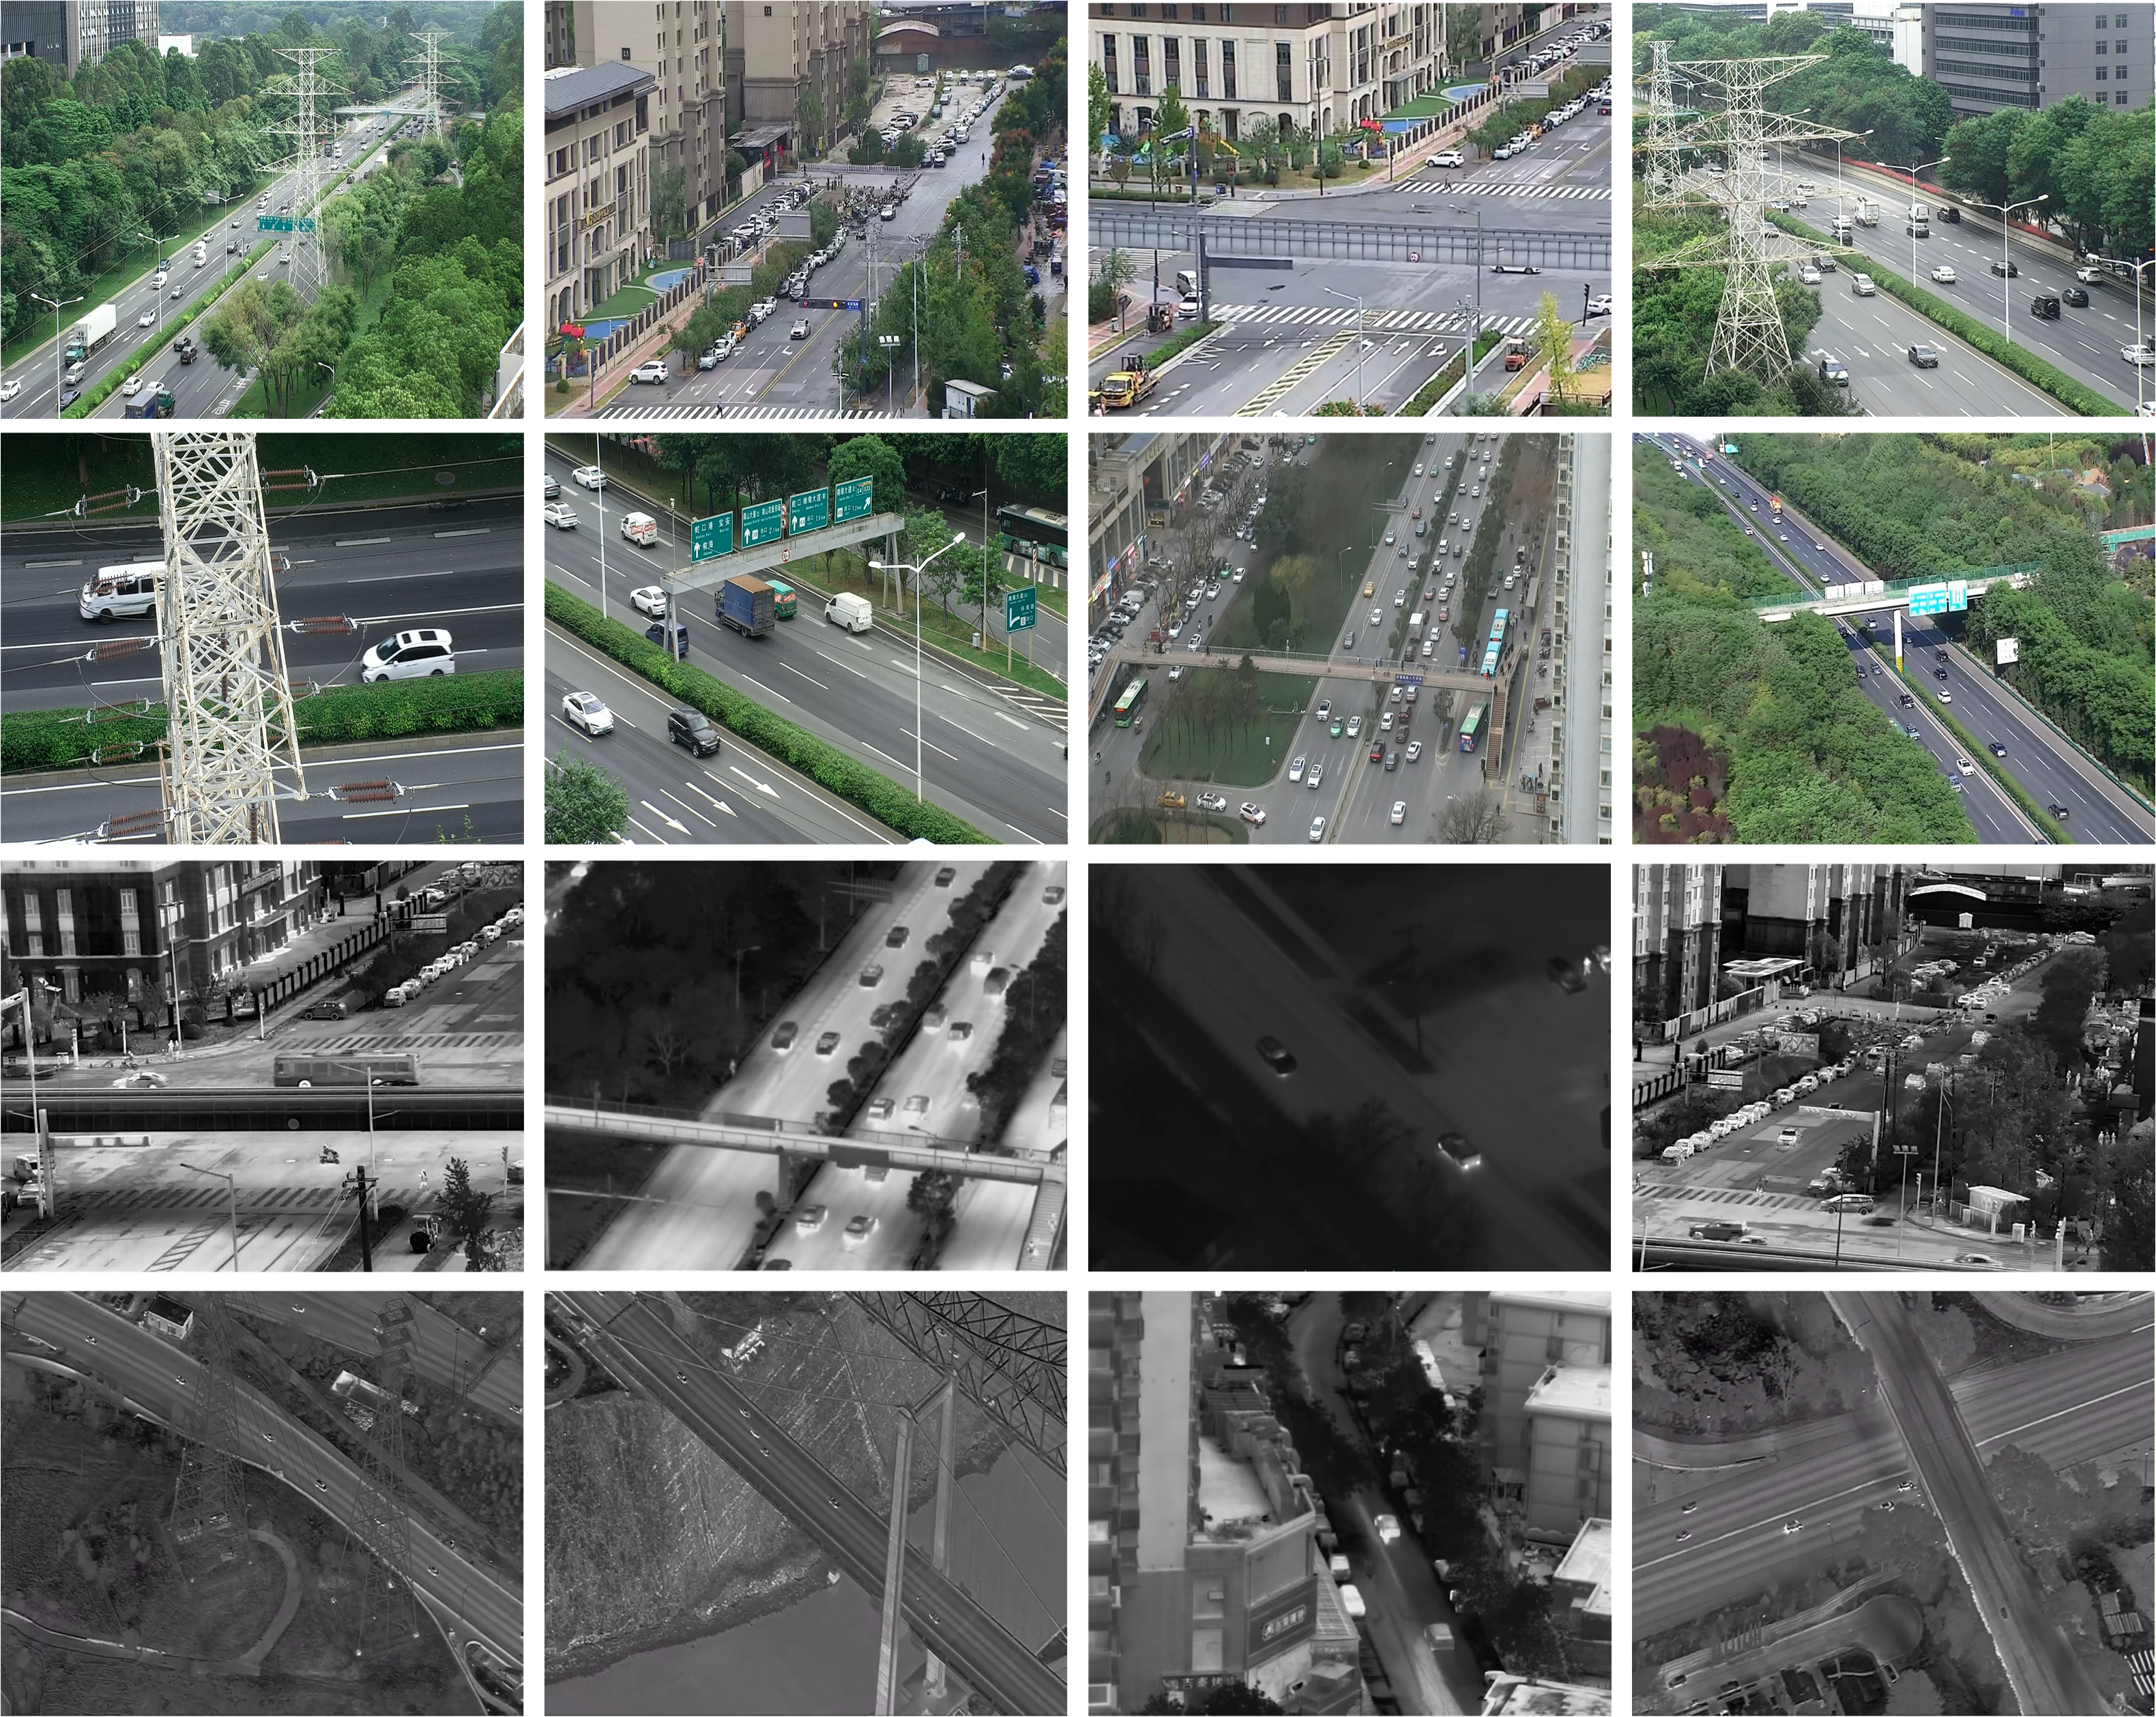
\includegraphics[width=0.8\textwidth]{mmuot.png}
    \caption{MMUOT-1050数据集示例}
    \label{mmuot}
\end{figure}

本文采用以边界框重合度为基础的成功率(Success Rate)作为评测指标。该指标能直观地衡量跟踪器在整个视频序列中持续、准确框定目标的能力。计算方式是首先计算每一帧的跟踪结果与真实标注之间的重叠率,然后统计整个序列中重叠率超过设定阈值的帧所占的比例来得到算法的成功率,重叠率与成功率的定义如下。
\begin{equation}
    \text{OR} = \frac{B_{pred} \cap B_{gt}}{B_{pred} \cup B_{gt}}
\end{equation}

\begin{equation}
    \text{Success Rate} = \frac{\mathcal{N}_{OR > \text{threshold}}}{\mathcal{N}_{total}}
\end{equation}

其中,$B_{pred}$为预测边界框,$B_{gt}$为真实边界框。OR值越大,表示跟踪器预测的边界框与真实边界框越接近。

\paragraph{实现细节}
为验证本文所提智能光电系统及算法的为验证本文所设计的智能光电系统及算法的实际效果,我们搭建了一套完整的飞行验证平台。该平台以大疆Matrice 350 RTK无人机作为飞行载体,本文设计的智能光电系统作为任务载荷,通过适配的云台接口与减震结构,被集成于无人机机身底部。系统硬件核心采用前文所述的瑞芯微RK3588边缘计算模组,同时接入可见光与红外相机,计算模组、传感器、电源管理模块及散热单元被集成于一个定制的轻量化壳体内,采用Microhard PX2作为数传模块,贴于机身外表面,整个系统如图\ref{djdrone}所示。
\begin{figure}[htbp]
    \centering
    \includegraphics[width=0.5\textwidth]{djdrone.png}
    \caption{飞行验证平台}
    \label{djdrone}
\end{figure}

在软件层面,完整的软件算法框架被部署于RK3588模组上,通过交叉编译与RKNN工具链优化,目标检测与跟踪算法被移植到模组上,数据处理层的算法与任务调度器作为后台服务常驻运行,系统与无人机飞控之间通过串口通信,与上位机通过PX2数传模块以udp协议通信。上位机实时显示相机拍摄到的画面,同时下发检测跟踪等指令。

验证飞行在多种具有代表性的城郊环境中进行,测试涵盖了包括复杂道路、密集建筑区及开阔场地在内的多种场景。系统主要跟踪高速运动的车辆,重点检验算法对快速目标运动及因树木、电线,天桥以及交通灯等造成的遮挡的鲁棒性。所有飞行测试均同步录制双光原始视频流,这些数据不仅直接用于系统的实时性能评估,也作为后期离线精细化分析的基础,并用以扩充和完善MMUOT-1050数据集。

\paragraph{实验结果}
为验证SKF-Tracker在无人机视角、遮挡频繁场景下的综合性能,我们在自建的MMUOT-1050数据集上,与多种在嵌入式平台上能够实时运行的代表性跟踪算法进行对比,包括经典的相关滤波算法(KCF、DSST、ECO)与基于深度学习的孪生网络方SiamRPN。所有实验均在RK3588模组上运行,相关滤波算法运行在CPU上,神经网络算法经过RKNN加速运行在NPU上。

\begin{table}[h!]
  \centering
  \caption{MMUOT-1050数据集结果}
  \label{trackres}
  \begin{tabular*}{0.75\textwidth}{@{\extracolsep{\fill}}lccc}
    \toprule
    \textbf{方法} & \textbf{可见光视频成功率} & \textbf{红外视频成功率} & \textbf{FPS} \\
    \midrule
    Baseline(KCF) & 75.37 & 80.2 & \textbf{33.93}\\
    DSST & 80.09 & 83.16 & 23.37\\
    ECO & 86.72 & 85.27 & 11.49\\
    SiamRPN & 88.49 & 88.52 & 15.31\\
    \textbf{SKF-Tracker} & \textbf{89.37} & \textbf{91.93} & 31.25 \\
    \bottomrule
  \end{tabular*}
\end{table}

实验结果如表\ref{trackres}所示,SKF-Tracker在跟踪精度上取得了最佳的综合性能。在可见光视频上,其成功率达到89.37\%,较ECO和SiamRPN分别提升了2.65\%和0.88\%,在更具挑战性的红外视频上,其优势更为显著,成功率达91.93\%,领先第二名SiamRPN3.41\%。在实时性方面,SKF-Tracker在保持最高精度的同时,仍能维持29.41 FPS的帧率,其速度远超基于深度神经网络的SiamRPN,并且只在CPU上运行,不占用NPU资源,与Baseline相比,虽然帧率略低,但是精度远高于Baseline(超过14\%),DSST和ECO在速度与精度上均落后于SKF-Tracker。实验结果表明SKF-Tracker在无人机视角下的遮挡频繁场景中,展现出了稳定的抗遮挡长时跟踪能力,达到了精度与实时性的良好平衡。


为了对比响应图峰值与SSIM在遮挡判定上的效果,我们选取具有典型完全遮挡-重现过程的视频序列,在本文SKF-Tracker框架下同步记录了目标被遮挡过程中,响应图峰值与SSIM值的变化情况,对它们的动态规律进行统计分析,结果如图\ref{ssimvspv}所示
\begin{figure}[htbp]
    \centering
    \includegraphics[width=\textwidth]{ssimvspv.png}
    \caption{响应图峰值与SSIM值变化对比}
    \label{ssimvspv}
\end{figure}

响应图峰值作为算法中间结果,其行为复杂且不稳定,难以构成可靠的遮挡判据,其变化呈现以下模式,当目标开始被遮挡时,峰值会随之下降,并在一段时间内达到该序列的最低点$PV_{low}$。然而,$PV_{low}$的数值在不同序列间差异巨大,一般在0.2至0.6之间波动,在达到$PV_{low}$后,峰值并不会稳定保持,可能在低位徘徊不超过5-10帧后,出现虚假回升,但此值低于遮挡前的正常水平,也可能持续缓慢降低,在少数情况下,峰值会恢复至接近遮挡前的水平。这种高度不一致性使得基于固定阈值的判定策略极易失效。与响应图峰值不同,SSIM的变化规律清晰且一致,一旦目标被遮挡,当前帧预测区域与模板之间的SSIM会在极短的时间内(通常不超过5帧)发生断崖式下降,其数值从跟踪正常时的接近1,迅速跌落至接近0,在整个遮挡持续期间,SSIM值稳定维持在接近0的低位水平。通过实验可以发现,SSIM能够对目标“消失”这一状态变化做出快速的反应,通过设定合理阈值,可以准确判定目标被遮挡的状态,随即触发模板保护与搜索机制,为抗遮挡长时跟踪提供基础。

图\ref{trackvis}展示了SKF-Tracker在典型遮挡场景下的跟踪可视化结果。在图中可以看到,目标在被电塔和广告牌完全遮挡后,SKF-Tracker成功识别出遮挡状态,并通过轨迹预测与动态搜索机制,在目标重新出现时准确地重捕获目标,保持了连续稳定的跟踪效果。

\xsection{本章小结}{Chapter Summary}
本章设计并实现了一套面向无人机平台的智能光电系统,系统硬件采用高性能低功耗的边缘计算模组,集成可见光与红外双传感器,具备强大的实时数据处理能力。软件架构采用模块化设计,包含数据接入层、数据处理层及通信总线,实现了系统功能的高效协同与灵活扩展。在此基础上,提出了一种面向边缘计算设备的抗遮挡长时跟踪框架SKF-Tracker,框架采用模块化设计,可复用于任何基础跟踪器,通过引入基于结构相似性的跟踪置信度评估机制,准确识别目标遮挡状态,并结合卡尔曼滤波的轨迹预测与动态搜索策略,实现了在资源受限环境下的鲁棒长时跟踪。实验结果表明,SKF-Tracker在自建的MMUOT-1050数据集上表现出优异的跟踪精度和实时性,为机载光电系统提供了一种实用、高效的抗遮挡跟踪解决方案。本章工作包括了核心算法创新与完整软硬件系统集成,通过工程实现与实验验证,在资源受限条件下构建高实时、高鲁棒的机载智能感知系统,实现了从关键技术创新到工程化落地验证的完整闭环。

\begin{figure}[tbp]
    \centering
    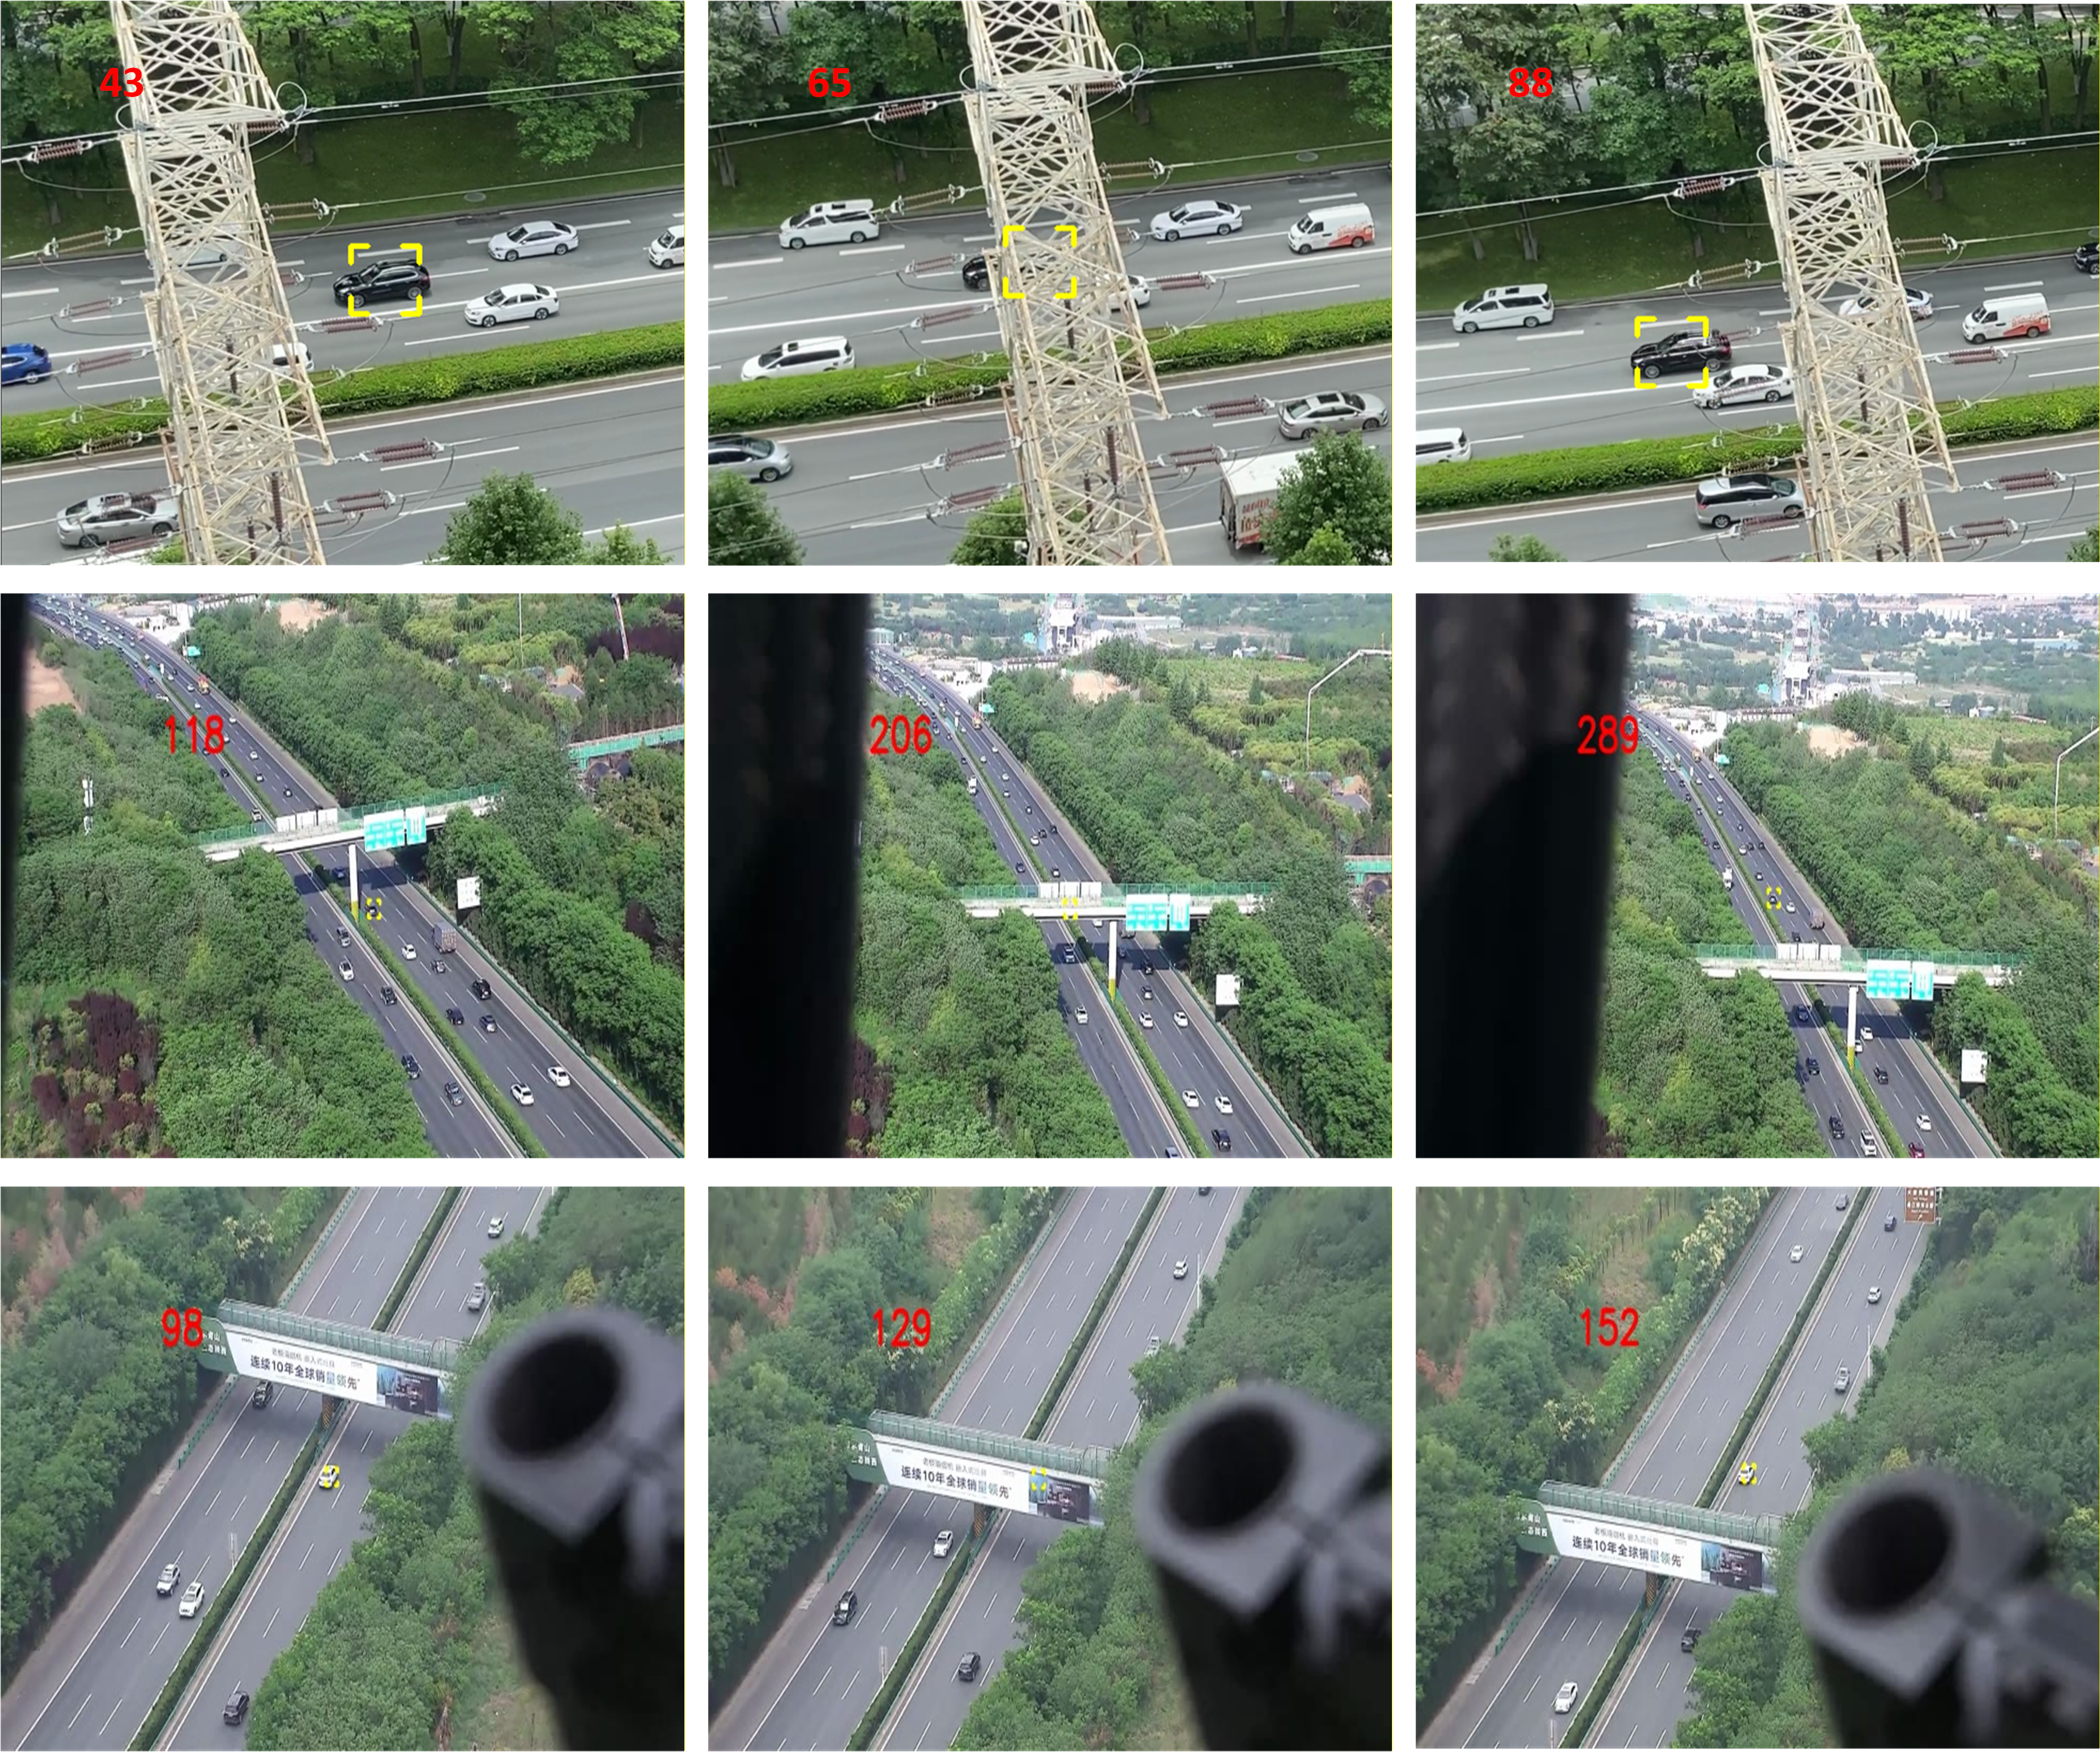
\includegraphics[width=0.9\textwidth]{trackvis.png}
    \caption{可视化结果}
    \label{trackvis}
\end{figure}




